% TODO: explain how depths are aligned to color images.
% TODO explain how tracking candidates are computed

\chapter{Derivations}
In this section we derive all necessary expressions that are required in order to implement our motion segmentation pipeline, which is described in the next chapter.

\section{Trajectory Affinities}
\label{sec:trajectory_affinities}
In this section we explain how we calculate similarities between extracted trajectories. This computation is the fundamental step of our work.
Before going into details, let us first revisit the definition of a trajectory. By the term trajectory we refer to a list of tracking points, which is ordered by the frame index in which each point was traced. Therefore, every points knows to which frame it belongs to. \\ \\
Let $A$, $B$ denote two trajectories resulting from the previous tracking step. Our goal is to define the similarity between the trajectories by computing a distance $d(A,B)$ between every trajectory pair. For that purpose we exploit their maximal dissimilarity via their maximal motion difference among all frames of common visibility. The squared version of this conceptual formula description is listed in equation $\ref{eq:prod_dist_affinity}$ 
\begin{equation}
	d^2 \left( A, B \right) = \max_t d_t^2 \left( A, B \right)
	\label{eq:product_distance}
\end{equation}
The resulting distance value from equation $\ref{eq:product_distance}$ is then turned into a affinity via the transformation
\begin{equation}
	w \left( A, B \right) = e^{ -\lambda d^2 (A, B) }.
	\label{eq:prod_dist_affinity}
\end{equation}
This measure is based on the work of Shepard $\cite{Shepard87}$ who proposed as a universal law that distance and perceived similarity are related via an exponential function.


where

\begin{equation}
	d_t^2 \left( A, B \right) = d_{spatial}^{A,B} \left( d_{motion}^{A,B} (t) \right) ^2
\end{equation}

\begin{equation}
	d_{spatial}^{A,B} = \frac{1}{\omega - \alpha + 1} \sum_{k=\alpha}^\omega \norm{A(k) - B(k)}
\label{eq:spatial_distance}	
\end{equation}
where $\alpha$ is the first- and $\omega$ is the last- overlapping frame index between the two given trajectories $A$ and $B$.

\begin{equation}
	d_{motion}^{A,B} \left( t \right)  = \frac{\norm{\partial_t A - \partial_t B}}{\sigma_t}
\label{eq:motion_distance}
\end{equation}
The expression $\partial_t A$ denotes the averaged motion over time, which is computed by approximating the derivatives $\partial_t A$, $\partial_t B$ using forward differences with a certain timestep $T$.

\begin{equation}
	\partial_t A = \frac{1}{T} \left( x_{t+T}^{A} - x_{t}^{A}, y_{t+T}^{A} - y_{t}^{A}\right)
\end{equation}
The exact value of $T$ is either the number of overlapping frames between the $A$ and $B$ or a fixed number, in case there are fewer common frames available, than a fixed threshold. \\ \\
Please note that by computing the affinity for every existing trajectory pair combinations, as defined in equation $\ref{eq:prod_dist_affinity}$, we implicitly encode a $n \times n$ affinity matrix $W$, for $n$ given trajectories. 

\section{Eigendecomposition of Graph Laplacians}
Given the pairwise affinity matrix $W$ as computed in section $\ref{sec:trajectory_affinities}$ on page $\pageref{sec:trajectory_affinities}$. An example of such an matrix is shown in figure $\ref{fig:cars_affinity_mat_sub}$. An approximated partitioning of the underlying graph can be obtained by running a variant of spectral clustering. Let
\begin{equation}
	D = \text{diag} \left( d_{A_1}, \dots, d_{A_n} \right)
\label{eq:def_d_mat}
\end{equation}
be the $n \times n$ diagonal matrix with the entries
\begin{equation}
	d_{A_k} = \sum_B w \left( A_k, B \right)
\end{equation}
The eigendecomposition of the normalized graph Laplacian is given by equation $\ref{eq:normalized_graph_laplacian}$.
\begin{equation}
	V^{T} \Lambda V = D^{-\frac{1}{2}} \left( D - W \right) D^{-\frac{1}{2}}
	\label{eq:normalized_graph_laplacian}
\end{equation}
Where $V$ denotes a matrix containing the column-wise eigenvectors of the Laplacian and $\lambda$ is a diagonal matrix containing the corresponding eigenvalues. Figure $\ref{fig:cars_eigenvectors_laplacian}$ shows two example eigenvectors, resulting from the $\textit{cars}$ dataset.

\begin{figure}[H]
\begin{center}
\subfigure[Eigenvector Front-Car]{
   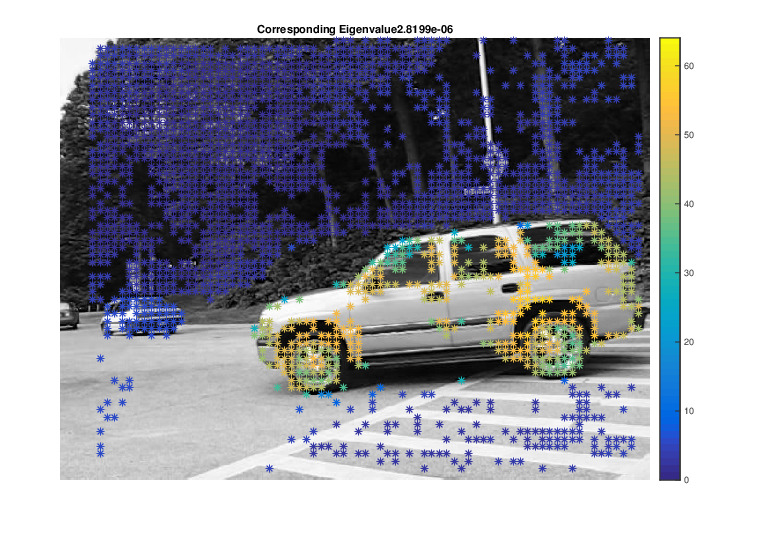
\includegraphics[width=0.48\linewidth] {derivation/eigenvectors/cars/ev_cf}
   \label{fig:cars_eigenvectors_laplacian_a}
}
\subfigure[Eigenvector Back-Car]{
   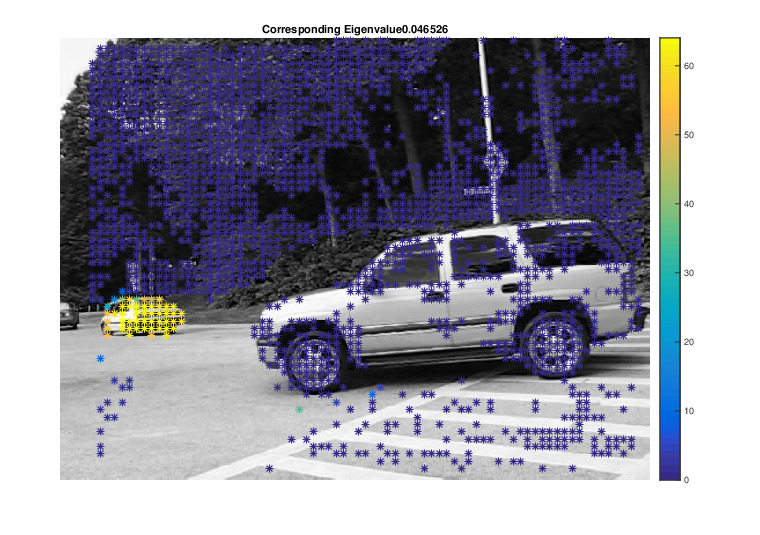
\includegraphics[width=0.48\linewidth] {derivation/eigenvectors/cars/ev_cb}
   \label{fig:cars_eigenvectors_laplacian_b}
}
\end{center}
\caption[Eigenvectors of the Laplacian]{Visualizing the contribution of two significant eigenvectors of the Laplacian of the affinity matrix that belong to the \textit{cars} dataset.}
\label{fig:cars_eigenvectors_laplacian}
\end{figure}

\begin{figure}[H]
\begin{center}
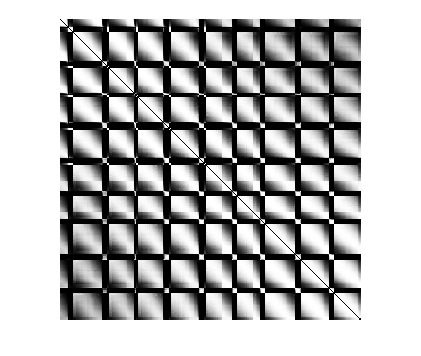
\includegraphics[width=0.7\linewidth] {derivation/eigenvectors/cars/w_mat}

\end{center}
\caption[Affinity Matrix W]{Visualization of the affinity matrix $W$ that belongs to the \textit{cars} dataset.}
\label{fig:cars_affinity_mat_sub}
\end{figure}
To obtain a simple segementation, we could run k-means on the first $k$ eigenvectors, that belong to the smallest k-eigenvalues. This approach yields a one-to-one mapping between cluster assignments and trajectory labels. However, the eigenvectors are often not piece-wise constant. Therefore, running k-means directly on the eigenvectors is not the best choice, since then the eigenvectors get approximated by multiple constant functions and thus the clustering yields an oversegementation. \\ \\
To address this issue we instead formulate a certain energy, containing a spacial regularity term that does not prefer spacial compact clusters. Moreover, it also takes edges in the eigenvectors into account. \\ \\
Let $v_i^A$ denote the $A-th$ component of the $i-th$ eigenvector in $V$ and $\bf{v}^A$ the vector composed of the $A-th$ components of the $m$ eigenvectors. Moreover, let $\mathcal{N}(A)$ denote the set of neighboring trajectories based on the spacial average distance. Then, we want to find the optimal cluster assignments $\pi^A \in {1, \dots, K}$ for a fixed, given number of clusters $K$, such that energy in equation $\ref{eq:min_cut_energy}$ gets minimized.	
\begin{equation}
\begin{aligned}
& E \left( \pi, K \right) = \sum_{A} \sum_{k=1}^K \delta_{\pi^A, k} \norm{\bf{v}^A - \mu_k}_{\lambda} + \nu \sum_A \sum_{B \in \mathcal{N}(A)} \frac{1- \delta_{\pi^A, \pi^B}}{\norm{\bf{v}^A - \bf{v}^B}} \\
& \text{where } \norm{\bf{v}^A - \bf{\mu}}_\lambda = \sum \frac{v_i^A -  \mu_i}{\lambda_i}
\end{aligned} 
\label{eq:min_cut_energy}
\end{equation}
The expression $\mu_k$ denotes the centroid of cluster $k$.

% TODO: explain the terms in the sum


\section{Minimum Cost Multicut Problem}



The min. cost multicut problem is the problem of decomposing a graph $G = (V, E)$ into an optimal number of segments such that the overall cost in term of of edge weights $c_e$ is minimized. The node labeling problem can equivalently be formulated as a binary edge labeling problem
\begin{equation}
\begin{aligned}
& \min_{y \in \{0,1 \}^{|E|}} \sum_{e \in E} c_e y_e \\
& \text{subject to } y \in MC
\end{aligned}
\end{equation}
where $MC$ is the set of all characteristic functions of all multicuts. This corresponds to all $y \in \{0,1 \}^{|E|}$ that form a closed boundaries, representing a valid decomposition of the graph. \\ \\
A formal decomposition of these characteristic functions can be described as the follows:
\begin{equation}
	\forall C \in \text{cycles}(G) \forall e \in C: y_e \leq \sum_{e^{'} \in C \backslash \{e\}} y_{e^{'}}
\end{equation}
It was shown, that is is sufficient to consider all chordless cycles, i.e. all cycles in which each node is only connected to its successor and predecessor. To avoid trivial solutions, the edge weights are typically chosen to be negative for edges that should be cut and positive for those connection nodes that should be joined. \\ \\
Given the cut probabilities $p_e$ of an edge $e \in E$, the negative of the \textit{logit} function 
\begin{equation}
	\text{logit}\left( p_e \right) = \log \left( \frac{p_e}{1 - p_e} \right)
	\label{eq:logit_function}
\end{equation}
provides such a behavior. A plot if the negative logit function defined as in $\ref{eq:logit_function}$ is shown in figure $\ref{fig:negative_logit_function}$.
\begin{figure}
\centering
\begin{tikzpicture}[trim axis left]
\begin{axis}[
  axis x line=center,
  axis y line=center,
  grid=both,
  xtick={-2,-1,...,1,2},
  ytick={-2,-1,...,1,2},
  xlabel={$x$},
  ylabel={$-\text{logit}\left( x \right)$},
  xlabel style={below right},
  ylabel style={above left},
  no markers,
  xmin=-0.5,
  xmax=1.5,
  ymin=-1.5,
  ymax=1.5]
\addplot +[thick, domain=0:1] {-log10(x/(1-x)};
\end{axis}
\end{tikzpicture}
\caption[Logit Function Plot]{A plot of the negative logit function applied on the domain [0,1].}
\label{fig:negative_logit_function}
\end{figure}
If $p_e < 0.5$ then $\text{logit}\left( p_e \right) > 0$ and thus the according edge cost $c_e$ is positive and therefore the edge $e$ is expensive to be cut out from the graph. Conversely, in case that $p_e > 0.5$ the negative logit function of $p_e$ is smaller than zero and thus it is beneficial to cut e. \\ \\
For computing pseudo-probabilities, we use the inverse of the logit function, the so called logistic function
\begin{equation}
	f(z) = \frac{1}{1 + \exp \left( -z \right)}.
	\label{eq:logistic_function}
\end{equation}
The input values we put into the function from equation $\ref{eq:logistic_function}$ are computed by the transformed trajectory distances $d$:
\begin{equation}
	z \equiv z(d) = \beta_0 + \beta_1 d
\end{equation}
The prior probability of cutting two trajectories is defined by the intercept value $\beta_0$. Assuming we learned $\beta_0$ for a certain prior cut probability $p$ and are given a new prior cut probability $\tilde{p}$, we can adapt the value $z$ by
\begin{equation}
	z = \beta_0 - \log \left( \frac{p}{1-p} \right) + \log \left( \frac{\tilde{p}}{1-\tilde{p}} \right) + \beta_1 d.
\end{equation}
If the cut prior is increased, more edges will be cut and the number of resulting segments increases. Small cut priors results in an undersegmentation. \\ \\
In the following we define a measure for the trajectory distances. This distances makes use of the motion-, spatial- and color distance of the overlapping segments between two trajectories $A$ and $B$. Note that the definition of the motion distance is given by equation $\ref{eq:motion_distance}$ and the spatial distance is given by the definition stated in equation $\ref{eq:spatial_distance}$. For the color distance we compute the average color within the overlapping frames using the CieLab\footnote{The key property of the Cie Lab color space is that its values are uniformly spaced. This allows us to use the l2 norm in order to compute meaningful color differences.} color space. More precisely, the color distances $d_{color}$ is defined as the follows:

\begin{equation}
	d_{color}^{A,B} = \frac{1}{\omega - \alpha + 1} \sum_{k=\alpha}^\omega \norm{\text{ColorAt}(k, A(k)) - \text{ColorAt}(k, B(k))}_2
	\label{eq:color_dist}
\end{equation}
where $ColorAt(k, A(k))$ yields the CieLab color value in frame $k$ at the image location $A(k)$\footnote{Remember that $A(k)$ denotes the tracking position of trajectory $A$ in frame $k$}.
The final trajectory distance is computed by combining the described distance values as in equation $\ref{eq:sum_dist}$.
\begin{equation}
\begin{aligned}
z ( A, B ) = \max (\tilde{\beta_0} & + \beta_1 d_{motion}^{A,B} \\
& + \beta_2 d_{spatial}^{A,B} \\
& + \beta_3 d_{color}^{A,B},\\
\beta_0 & + \beta_1 d_{motion}^{A,B} )
\end{aligned}
\label{eq:sum_dist}
\end{equation}
If the sum of the spatial and the color distance is large in equation $\ref{eq:sum_dist}$ then only the motion distances are considered. This ensures that trajectories which are far apart but move similarly still end up in the same segment.

\section{Hole Filling}
\label{section:hole_filling}
In this section we address the problem of \emph{Hole Filling} by formulating this problem as a convex optimization. This formulation should enable us to generate dense segmentations from sparse segmentations. For solving the problem we develop and apply a primal-dual approximation. 
Given an image $g$ has missing information in form of holes, we want to find an optimal reconstructed image $u$. For describing the optimality property we take into account a cost function that describes the color smoothness and also that the resulting image $u$ should be close to the given raw input image $g$. \\ \\
More precisely, let $g$ denote a color image that exhibits holes. Then we want to solve for $u=(u_r, u_g, u_g)$ (RGB image) by minimzating the following energy term (cost function):
\begin{align}
	E(u_c) = \norm{\nabla u_c}_2 + \frac{\lambda}{2} \norm{u_c - g}^2_{\Omega_{c}}
\label{eq:basis_cost_demosaicing}	
\end{align}
with the measure
\begin{equation}
	\norm{u_C - g}^2_{\Omega_{C}} = \sum_x \sum_y \Omega_{C}(x,y)\norm{u_{c}(x,y) - g(x,y)}^2
\label{eq:measure}
\end{equation}
where C denotes the three different color channels. $\Omega_{C}$ is defined such that $\Omega_{C}(x,y) = 1$ if the pixel value at $(x,y)$ is \emph{valid}$\footnote{this means that the pixel at location (x,y) is valid for the bayer color mask C}$ and $\Omega_{C}(x,y) = 0$ when the data is missing. \\ \\
The cost function from equation $\ref{eq:basis_cost_demosaicing}$ consists of a smoothness term, $\norm{\nabla u_c}_2$ and $\norm{u_c - g}^{2}_{\Omega_{c}}$. The first term ensures a smooth color transition between colors in a l2 norm sense. The second term ensures that the reconstructed images does not deviate too much from the given input, i.e. de demosaiced image should resemble to the provided mosaiced raw camera image. This similarity term is further parameterized by a regularization term $\lambda$, indicating how strong the output should match the given input according to the formulated measure in equation $\ref{eq:measure}$. In summary, larger values for $\lambda$ weight the similarity of the input and output image more, and contrarely, lower values weight the color smoothness term more. \\ \\
Hereby, minimizating the cost function from equation $\ref{eq:basis_cost_demosaicing}$ leads to an optimal demosaiced image $u$.
Mathematically we want to solve for 

\begin{equation}
	\widetilde{u} = \argmin_{u_c} E(u_c)
\label{eq:our_general_cost_function}
\end{equation}
We can further simplify the cost function stated in equation $\ref{eq:basis_cost_demosaicing}$ relying on the following observation: Since the function $\Omega_{C}$ is only true for pixels that correspond to the color channel C in the bayer mask, we see that 
\begin{equation}
	\Omega_{C}(x,y)\norm{u_{c}(x,y) - g(x,y)}
\end{equation}
is only not equal zero if the pixel at location $(x,y)$ belongs to the color channel $C$. Therefore we are allowed to solve the stated optimization problem from equation $\ref{eq:basis_cost_demosaicing}$ for each color channel separately. 


According to this insight we are supposed to minimize the following three independent$\footnote{Independent in the sense that we are allowed to solve for each color channel separately}$ convex problems:



\begin{align}
	\widetilde{u}_R = \argmin_{u_R} \norm{\nabla u_R}_2 + \frac{\lambda}{2} \norm{u_R - g}^2_{\Omega_{R}} \nonumber \\
	\widetilde{u}_G = \argmin_{u_G} \norm{\nabla u_G}_2 + \frac{\lambda}{2} \norm{u_G - g}^2_{\Omega_{G}}\nonumber \\
	\widetilde{u}_B = \argmin_{u_B} \norm{\nabla u_R}_2 + \frac{\lambda}{2} \norm{u_B - g}^2_{\Omega_{B}}
\label{eq:our_convex_probelm}		
\end{align}

Where we still rely on the measure defined in equation $\ref{eq:measure}$ but C was replayed by the appropriate color channel$\footnote{C stands for either the color channel R, G or B.}$. We notice that the equations in $\ref{eq:our_convex_probelm}$ tell us that we have to solve three different energies similar to the one formulated in equation $\ref{eq:our_general_cost_function}$.

In the next section we will describe how to solve the stated minimization problems from equation $\ref{eq:our_convex_probelm}$ numerically.

\subsection{Primal-Dual Form}
In this section we derive the primal-dual form of the stated convex demosaicing problem.

But first off, let us consider an initial problem of the form 

\begin{align}
	\min_{x \in X} F(K x) + G(x)
\label{eq:initial_primal}	
\end{align}

where $F$, $G$ are convex functions and $K$ denotes a linear operator. 

The primal-dual formulation for equation $\ref{eq:initial_primal}$ is given by 

\begin{align}
	\min_{x \in X} \max_{y \in Y} < Kx, y > - F^*(y) + G(x)
\label{eq:initial_primal_dual}	
\end{align}


For a given mosaiced RGB image $u_{RGB}$ encoded as a 3 dimensional $M \times N$ matrix, i.e. a tensor of dimension $M \times N \times 3$. As mentioned in the problem statement we can solve three independent convex problems in order to solve the problem of demosaicing a RGB image. Therefore let in the following $u$ define stand for one particular color channel of the given color image $u_{RGB}$.

\begin{equation}
\min_{u \in U} \norm{\nabla u} + \frac{\lambda}{2} \norm{u - g}^2_{\Omega}
\label{eq:initial_energy}
\end{equation}

where $\norm{u - g}^2_{\Omega}$ is defined as in equation $\ref{eq:measure}$ and $g$ is the corresponding color channel of the mosaiced image described in the problem statement.

We observe that equation $\ref{eq:initial_energy}$ has the same structure as the initial problem stated in equation $\ref{eq:initial_primal}$. This allows us to formulate the primal-dual form of equation $\ref{eq:initial_energy}$ which will look like the following:

\begin{align}
	\min_{u \in U} \max_{y \in Y} < Kx, y > - F^*(y) + G(x)
\label{eq:initial_primal_dual}	
\end{align}

Where $K$, $F$ and $G$ are defined as:

\begin{align}
	K &= \nabla \nonumber \\
	F &= \norm{\cdot}_2 \nonumber \\
	G &= \norm{u - g}^2_{\Omega}
\label{eq:def_kfg}	
\end{align}

Note that $F*$ denotes the convex conjugate form of $F$. The convex conjugate of $F$ has an explicit identity that can be computed using the Legendre-Fenchel-Transform.

\begin{align}
	F^*(y) &= (\norm{\cdot}_2)^*(y) \nonumber \\
		  &= \sup_x x^T y - \twonorm{x} \nonumber \\
		  &= \sup_x x^T y - \max_{\twonorm{z} \leq 1} x^T z \nonumber \\
		  &= \sup_x \min_{\twonorm{z} \leq 1} x^T(y-z) \nonumber \\
		  &= \begin{cases}
   				0  			& \text{if} \twonorm{y} \leq 1 \\
   				\infty      & \text{otherwise}
  			 \end{cases} \nonumber \\
  		  &= \delta(y)
\label{eq:legendre_fenchel_transform_f}  		  
\end{align}

The first equality is simply the definition of $F$. The second equality is using the so called Legendre-Fenchel transformation,

\begin{equation}
	(\norm{\cdot}_2)^*(y) = \sup_x x^T y - \twonorm{x} \nonumber
\end{equation}. 

In the third equality I make use of the Cauchy-Schwarz inequality, 
\begin{equation}
	\twonorm{x} = \max_{\twonorm{z} \leq 1} x^T z
\end{equation}


Plugging equation $\ref{eq:legendre_fenchel_transform_f}$ and the definitions in from equation $\ref{eq:def_kfg}$ into the primal-dual equation equation $\ref{eq:initial_primal_dual}$ we conclude the following final primal-dual formulation:

\begin{equation}
\min_{u \in U} \max_{y \in Y} <\nabla u, y> - \delta(y) + \frac{\lambda}{2}\norm{u - g}^2_{\Omega}
\label{eq:final_primal_dual}
\end{equation}


\subsection{Primal-Dual steps}
In this section I will present an iterative solver for our stated primal-dual formulation.

In the following I am going to rely on an algorithm $\cite{chambolle2011first}$ formulated by A.Chambolle and T.Pocke, which allows to solve primal-formulations as ours stated in equation $\ref{eq:final_primal_dual}$.
They stated an iterative algorithm that has the following update steps:

\begin{align}
	y^{n+1} &= \prox_{\sigma F^*}(y^n + \sigma K \bar{x}^n) \nonumber \\
	x^{n+1} &= \prox_{\tau G}(x^n - \tau K^* y^{n+1}) \\
	\bar{x}^{n+1} &= x^{n+1} + \theta(x^{n+1} - x^n)
\label{eq:update_rules_plain}	
\end{align}
with $\theta \in (0, 1]$ and the constraint $\tau \sigma \norm{K}^2 < 1$. Note that stated constraint is important in order to guarantee convergence of their algorithm.

Hereby $prox(\cdot)$ denotes the proximity operator and is defined as 

\begin{equation}
	\prox_{\lambda F}(z) = \arg \min_x \frac{1}{2} \twonorm{x - z}^2 + \lambda F(x)
\end{equation}

In the following we will derive explicit identities for the update rules in equation $\ref{eq:update_rules_plain}$that can be numerically solved. Our goal is to find an expression for the proximity operator.

\subsection{Update for $y^{n+1}$}

In this subsection we derive an identity for the $y^{n+1}$ update rule from equation $\ref{eq:update_rules_plain}$. The key idea is to use the so called Moreau's Identity:  

\begin{equation}
	\prox_{\lambda F^*}(z) = z - \lambda \cdot \prox_{F/ \lambda}(z / \lambda) 
\label{eq:moreau}	
\end{equation}

Next, we apply the Moreau's identity to the proximity operator of the Legendre-Fenchel transformation.


\begin{align}
	\prox_{\lambda F^*}(y^n + \sigma K \bar{x}^{n}) 
	&= (y^n + \sigma K \bar{x}^{n}) - \sigma \prox_{\frac{F}{\sigma} } \left(\frac{y^n + \sigma K \bar{x}^{n} }{\sigma} \right) \nonumber \\
	&= (y^n + \sigma K \bar{x}^{n}) - \sigma \left( \frac{y^n + \sigma K \bar{x}^{n} }{\sigma} \max{0, 1-\frac{1}{\twonorm{y^n + \sigma K \bar{x}^{n} }}} \right) \nonumber \\
	&= (y^n + \sigma K \bar{x}^{n}) - \left( y^n + \sigma K \bar{x}^{n} \right) \max{\left(0, 1-\frac{1}{\twonorm{y^n + \sigma K \bar{x}^{n} }}\right)}  
\label{eq:y_n_1_expression}
\end{align}

For the first equality we use the definition of equation $\ref{eq:moreau}$ and for the second equality we used the fact (proven during class) that

\begin{align}
	\prox_{\frac{\twonorm{\cdot}}{\sigma}}(\frac{x}{\sigma}) = \frac{x}{\sigma} \max{\left(0, 1-\frac{1}{\twonorm{x}}\right)}
\end{align}

To simplify our derivation even and also get rid of the proximity operator we next make a case distinction for $\twonorm{y^n + \sigma K \bar{x}^{n}}$. 

\begin{itemize}
	\item If $\twonorm{y^n + \sigma K \bar{x}^{n}} \geq 1$
		then  
		\begin{align}
			0 \leq 1-\frac{1}{\twonorm{y^n + \sigma K \bar{x}^{n}}} \leq 1
		\end{align}
		
		Therefore $\frac{1}{\twonorm{y^n + \sigma K \bar{x}^{n}}}$ is smaller than one and thus
		
		\begin{align}
			\max{\left(0, 1-\frac{1}{\twonorm{y^n + \sigma K \bar{x}^{n}}}\right)} 
			&= 1-\frac{1}{\twonorm{y^n + \sigma K \bar{x}^{n}}}
		\end{align}
		
		This insight can directly be used for the maximum expression in equation $\ref{eq:y_n_1_expression}$ and we hence obtain:
		
		\begin{align}
			\prox_{\lambda F^*}(y^n + \sigma K \bar{x}^{n})
			&= (y^n + \sigma K \bar{x}^{n}) - \left( y^n + \sigma K \bar{x}^{n} \right) \max{\left(0, 1-\frac{1}{\twonorm{y^n + \sigma K \bar{x}^{n} }}\right)} \nonumber \\
			&= (y^n + \sigma K \bar{x}^{n}) - \left( y^n + \sigma K \bar{x}^{n} \right) \left( 1-\frac{1}{\twonorm{y^n + \sigma K \bar{x}^{n}}} \right)\nonumber \\
			&= (y^n + \sigma K \bar{x}^{n}) -(y^n + \sigma K \bar{x}^{n}) +\frac{y^n + \sigma K \bar{x}^{n}}{\twonorm{y^n + \sigma K \bar{x}^{n}}} \nonumber \\
			&= \frac{y^n + \sigma K \bar{x}^{n}}{\twonorm{y^n + \sigma K \bar{x}^{n}}}
		\end{align}
		
	\item If $\twonorm{y^n + \sigma K \bar{x}^{n}} < 1$
		then 
		\begin{align}
			1-\frac{1}{\twonorm{y^n + \sigma K \bar{x}^{n}}} < 0
		\end{align}
		thus we conclude 
		\begin{align}
			\max{\left(0, 1-\frac{1}{\twonorm{y^n + \sigma K \bar{x}^{n}}}\right)} 
			&= 0
		\end{align}
		which offers us the following new identity for equation $\ref{eq:y_n_1_expression}$:
		
		\begin{align}
			\prox_{\lambda F^*}(y^n + \sigma K \bar{x}^{n})
			&= (y^n + \sigma K \bar{x}^{n}) - \left( y^n + \sigma K \bar{x}^{n} \right) \max{\left(0, 1-\frac{1}{\twonorm{y^n + \sigma K \bar{x}^{n} }}\right)} \nonumber \\
			&= (y^n + \sigma K \bar{x}^{n}) - \left( y^n + \sigma K \bar{x}^{n} \right) 0 \nonumber \\
			&= y^n + \sigma K \bar{x}^{n}
		\end{align}
\end{itemize}

By using the results from the case distinction from above we can simplify equation $\ref{eq:y_n_1_expression}$ even further to:

\begin{equation}
	\prox_{\lambda F^*}(y^n + \sigma K \bar{x}^{n}) = \frac{y^n + \sigma K \bar{x}^{n}}{\max{\left(1,\twonorm{y^n + \sigma K \bar{x}^{n}} \right)}}
\label{eq:y_p_1_we_proxy}	
\end{equation}

Finally, the only left step to do is to plug in the definition of $K$ into equation $\ref{eq:y_p_1_we_proxy}$ which gives us then the final update rule for $y_{n+1}$ when relying on the update rule from equation $\ref{eq:y_n_1_expression}$:

\begin{align}
	y_{n+1} = \frac{y^n + \sigma \nabla \bar{x}^{n}}{\max{\left(1,\twonorm{y^n + \sigma \nabla \bar{x}^{n}} \right)}}
\label{eq:update_rule_y_n_p_1}	
\end{align} 	

\subsection{Update for $x^{n+1}$}

\begin{align}
x^{n+1} &= \prox_{\tau G}(x^n - \tau K^* y^{n+1}) \\
		&= \prox_{\tau \frac{\lambda}{2} \norm{u - g}_{\Omega}^2 }(x^n - \tau \nabla^* y^{n+1}) \\
	    &= \arg \min_{z} \frac{1}{2} \twonorm{\left(x^n - \tau \nabla^* y^{n+1} \right) - z}^2 + \tau \frac{\lambda}{2}\norm{z - g}_{\Omega}^2 \\
	    &= \arg \min_{z} E(z)
\label{eq:energy_x_p_1}	    
\end{align}

To simplify the following derivations, let us define the following substitution: 
\begin{align}
	m := \left(x^n - \tau \nabla^* y^{n+1} \right)
\end{align}

We can solve for $x^{n+1}$ by finding the zeros of the partial derivative of $E(z)$ from equation $\ref{eq:energy_x_p_1}$. Let us start with the partial derivative along $z$ of $E(z)$ from equation $\ref{eq:energy_x_p_1}$: 

\begin{align}
	\partial_{z} E(z)
	&= \partial_{z} \left( \frac{1}{2} \twonorm{m - z}^2 + \tau \frac{\lambda}{2}\norm{z - g}_{\Omega}^2 \right) \nonumber \\
	&= \frac{1}{2} \partial_{z} \left[ \left( m - z \right)^{T}\left( m - z \right) + \tau \lambda \Omega \left( z -g \right)^{T}\left( z -g \right) \right] \nonumber \\
	&= \frac{1}{2} \partial_{z} \left[ m^{T}m -2m^{T} z + z^{T} z + \tau \lambda \Omega \left( z^{T}z -2z^{T} g + g^{T} g\right) \right] \nonumber \\
	&= \frac{1}{2} \left[ -2m + 2z + \tau \lambda \Omega \left( 2 z -2g \right) \right] \nonumber \\
	&= \left[ -m + z + \tau \lambda \Omega z - \tau \lambda \Omega g \right]	 \nonumber \\	
	&= \left[ \left(1+\tau \lambda \Omega \right)z-m - \tau \lambda \Omega g \right]	 \nonumber \\
\label{eq:derivative_x_n_p_1}		
\end{align}

Next, let us set the finding from equation $\ref{eq:derivative_x_n_p_1}$ to zero and solve for $z$:

\begin{align}
	\partial_{z} E(z) 
	&= 0 \nonumber \\
	&\Leftrightarrow \left(1+\tau \lambda \Omega \right)z-m - \tau \lambda \Omega g = 0 \nonumber \\
	&\Rightarrow z = \left(m +  \tau \lambda \Omega g \right) \left( 1+\tau \lambda \Omega\right)^{-1} \nonumber \\
	&\Rightarrow z = \frac{m +  \tau \lambda \Omega g}{1+\tau \lambda \Omega} \nonumber \\
\label{eq:zeros_ez}	
\end{align}

Note that the division $(1+\tau \lambda \Omega)$ denotes a component-wise division, since $\Omega$ is applied component-wise to the elements of $g$. In addition, 1 and $\Omega$ are representing matrices here (of same dimension as $g$ and $z$ ($u$ respectively).

By plugging the definition $m$ into equation $\ref{eq:zeros_ez}$ and using the fact, that $z$ corresponds to $x^{n+1}$ we can conclude:

\begin{align}
	x^{n+1} 
	&= \frac{x^n - \tau \nabla^* y^{n+1} +  \tau \lambda \Omega g}{1+\tau \lambda \Omega} \nonumber \\
	&= \frac{x^n + \tau div(y^{n+1}) +  \tau \lambda \Omega g}{1+\tau \lambda \Omega}
\label{eq:update_x_n_p_1}	
\end{align}

In the last step we used the well known fact, that 
\begin{align}
	\nabla^* (v) = -div(v)
\end{align}

for any vector-field $v$ of the form 

\begin{align}
	v = \nabla u
\end{align}
 
